\documentclass[11pt, dvips]{report}
\usepackage[norsk]{babel}
\usepackage[latin1]{inputenc}
\usepackage{graphicx}

\begin{document}
\thispagestyle{empty}
\begin{center}
\LARGE{Multimedieprosjekt:\\
\bf Spill ved bruk av\\
OpenGL og 3D Studio}

\vspace{2em}
\begin{figure}[!h]
\center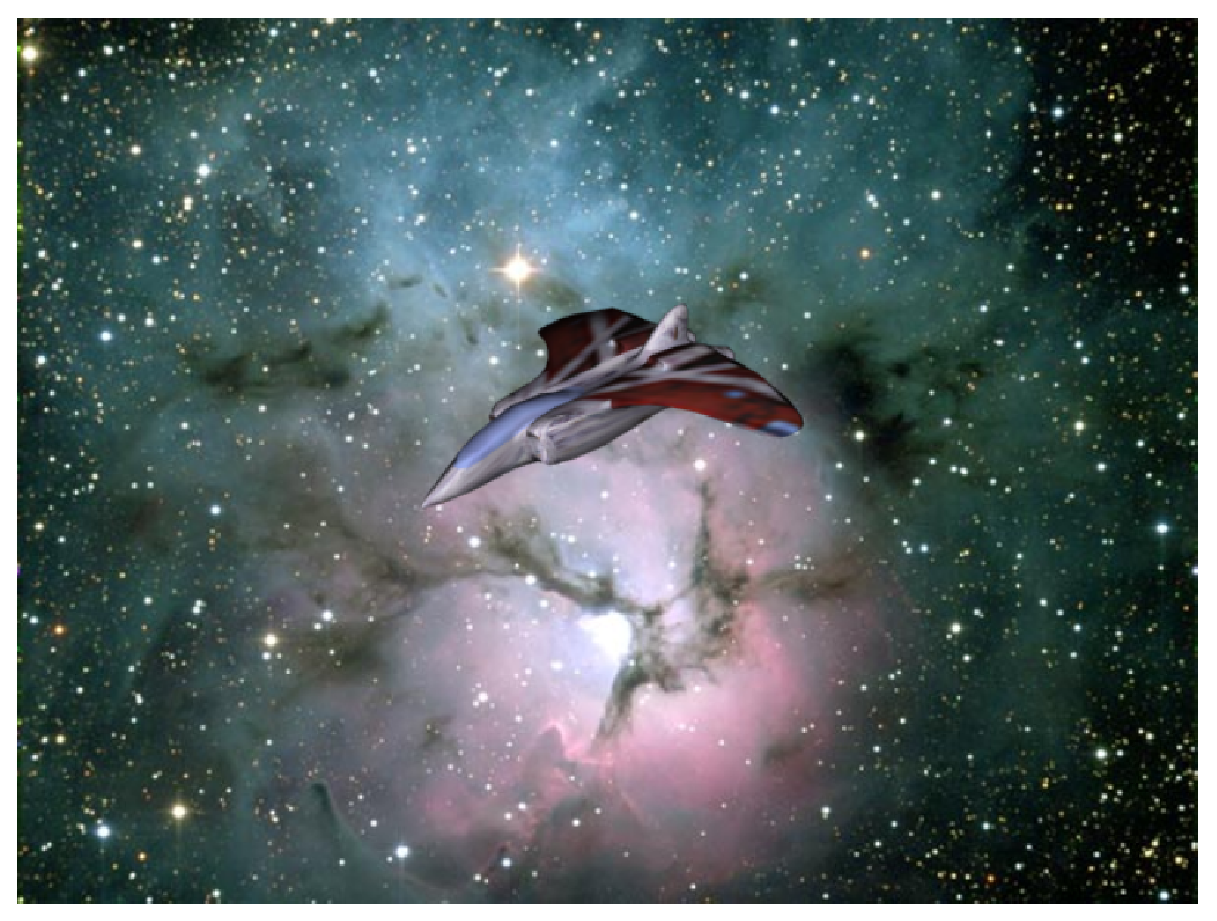
\includegraphics[width=10cm]{loading.eps}
\end{figure}
\vspace{2em}
\large{Tor Arvid Lund \qquad Nils Johan Torp \qquad Morten Wiig}\\[1em]
\today
\end{center}
\newpage

\begin{abstract}
Vi har laget et lite spill der man styrer et romskip i en 3D-verden.
Målet med dette spillet er å komme seg ut den hemmelige utgangen.
Denne åpner seg når du har samlet sammen alle krystallene på brettet.

3D-verdenen er modellert i 3D Studio Max. Vi har brukt C/C++ som
programmeringsspråk, og tilleggsbibliotekene OpenGL og SDL.
\end{abstract}

\tableofcontents

\chapter{Introduksjon} 

\section{Idéen}

Idéen til dette spillet kom fra et gammelt spill til Macintosh som het
Crystal Quest. Ingen av oss har noen gang hatt en Macintosh, men det
finnes noe lignende til PC (DOS) som heter XQuest. Det er et 2D-spill
der man skal samle krystaller på et enkelt, rektangulært brett, mens
man unngår steiner og monstre på brettet.

Måten man styrer dette skipet på er det som gjør spillet spesielt. Man
forflytter seg med musa, men man endrer \emph{farten}, og ikke
\emph{posisjonen}. Dette betyr at når man gir musa et puff, vil skipet
få litt fart, og deretter beholde denne farten til man dytter musa i
en annen retning (eller til man treffer en vegg, en stein, eller et
monster og dør...).

\section{Hvordan vi begynte}

Vi kunne ingenting om OpenGL eller grafikkprogrammering i det hele
tatt da vi begynte. Vi kunne heller ingenting om SDL eller
lydprogrammering. Vi var mao ganske nervøse, og ikke sikre på om vi
greide å hale dette i land, men det ser ut til å ha gått nogenlunde
greit.

\section{Åpen kildekode}

Vi benyttet oss av sider på nettet som tok for seg: ``OpenGL for de som
ikke kan noe fra før'' og det var meget lærerikt. Vi vil også gi ut
dette spillet som åpen kildekode (når jeg får ryddet litt i koden...)
under GNU Software Foundation sin GPL (General Public License).

\section{Bibliotek}

\subsection{OpenGL}

OpenGL (Open Graphics Library) er en grafikk-API utgitt av SGI
(Silicon Graphics Incorporated). Vi har valgt denne av den enkle grunn
at det stod mellom den og Direct3D. Direct3D er Microsofts
grafikk-API. Direct3D er lukket og låst til windows-plattformen. Den
får også hets, av programmerere som har brukt begge deler, for å være
rotete og uoversiktlig i forhold til OpenGL.

\subsection{SDL}

SDL (Simple DirectMedia Layer) er et bibliotek som hjelper oss med
mange ting. Det tar seg av input-håndtering (mus/tastatur), lyd,
timing, multithreading, nettverkskommunikasjon, etc. I tillegg er
biblioteket tilgjengelig på flere plattformer (Linux, Windows, BeOS,
Macintosh, ...), og det er i prinsippet mulig å lage
plattformuavhengige programmer i C/C++

\section{Programmeringsspråk}

Mange velger språk som Java eller til og med Visual Basic fordi de er
enkle å programmere i. Vi valgte C/C++ fordi det går meget raskt i
forhold til f.eks Java/VB. De som har sett Java3D applikasjoner kontra
C/C++ applikasjoner vet dette.

\section{Plattform}

Morten, som lager 3D-modellene, og Nils Johan, som lager modell-loader
og effekter er windows-gutter, mens jeg, Tor Arvid, er
Linux-forkjemper. Så, programmet vårt har forsåvidt blitt utviklet på
to plattformer, men det har blitt sammensatt og testet på Linux.

Vi prøvde å kompilere det på windows ved et tidlig stadium, og det
gikk fint. Den eneste forutsetningen når man kjører programmet, er at
i windows \emph{\bf{må}} man kjøre fullscreen, ellers går det
ufattelig seint.

Vi prøvde også rett før dette ble skrevet, å kompilere det ferdige
produktet i windows. Det går uten feil, men nå går det fryktelig seint
i windows. Vet ikke hvorfor, men jeg skal prøve å fikse opp i det en
av de nærmeste dagene.

\chapter{Planlegging}

\subsubsection{2D $\rightarrow$ 3D}

Når vi skulle lage \emph{vårt} program, var jo den store forandringen
fra XQuest at det skulle være 3 dimensjoner i stedet for bare 2.

Vi kunne da ikke gi skipet fart i alle tre dimensjonene med ei mus, og
bestemte derfor at musa skulle bestemme retningen vi ``kikket'' i, og
en tast på tastaturet skulle være ``gasspedalen''. Vi har også taster
for å rotere flyet om sin egen ``kikkeakse''.

Det som ble resultatet her, var et fly som var så godt som umulig å
styre. Når flyet kom opp i fart, var det umulig å stanse, fordi man
måtte snu seg i akkurat motsatt retning og gi gass. Denne retningen
klarer man så godt som aldri å finne.

Løsningen ble å legge inn en ``rygge-knapp'' (om enn meget lite
realisitisk), og friksjon, slik at når man slipper gassen, minker
farten sakte men sikkert.

\subsubsection{Kamera}

Hvordan kameraet skulle forholde seg til det som skjedde i 3D-verdenen
var litt vanskelig å bestemme seg for. Det ideelle er (synes vi) at
kameraet ligger bak flyet. Men hvis vi flytter eller roterer kameraet
akkurat når flyet gjør det, vil vi miste 3D-følelsen i spillet.
Kameraet trenger derfor en forsinkelse for å gjøre bevegelsene mer
realistisk. Mer om dette i kapittel \ref{camera}

\subsubsection{3D-Modeller}

Man kan legge inn koordinater direkte i OpenGL ved å taste inn
numeriske verdier for hver x/y/z koordinat, men vi bestemte oss
(selvfølgelig) for å lage modeller av skip, brett, asteroider og
krystaller i 3D Studio. Mer om det i kapittel \ref{3dmodel}.

\subsubsection{Lasting av modellene}

Når vi \emph{ikke} skriver inn koordinat-verdier direkte i OpenGL,
måtte vi ha en metode for å laste inn 3D Studio-modellene (.3DS filer)
i programmet. Vi trengte mao en .3DS-loader. Mer om denne i kapittel
\ref{3dload}.

\subsubsection{Kollisjonsdeteksjon}

Når skipet treffer en vegg, asteroide eller krystall, må programmet
vårt skjønne det på en eller annen måte. Dette var en av de
vanskeligste delene av prosjektet. Brettet er stort. Det inneholder
mellom 60000 og 100000 flater, og skipet har i underkant av 2000
flater. For å sjekke nøyaktig etter kollisjoner, må vi gå gjennom ei
løkke 200 millioner ganger (i verste fall).

Det sier seg selv, at her må vi jukse. Mer om dette i kapittel
\ref{collision}.

\subsubsection{Effekter}

Et hvert spill blir kjedelig uten effekter. Det ble ikke mye tid igjen
til å lage mye av dette, men vi har da en partikkel-eksplosjon og litt
lydeffekter. I tillegg har vi egenkomponert bakgrunnsmusikk (Muligens
dette tiårets minst spennende sang, men likevel...). Mer om effekter i
kapittel \ref{fx}

\chapter{Kamera}\label{camera}

Når vi tegner en 3D-verden i OpenGL, tegner vi alt i forhold til
kameraets plassering. Når kameraet skal forsinkes, blir det lett å
``gå i surr''. Det vi prøvde, var å lage et buffer til kameraet som
inneholdt de nødvendige vektorer for å plassere det riktig. Vi gjorde
dette bufferet stort nok til å holde informasjon om de 40 siste
frames.

Men vi ville at skipet skulle rotere i det øyeblikk man beveget musa,
så vi lagde et buffer til skipet også. Det som ble problemet her, var
at når man roterer kameraet, roterer også alle objektene i verdenen
tilsvarende. Det vil si at hvis man f.eks roterer skipet 90 grader mot
høyre, vil man se rotasjonen på skipet umiddelbart, men når kameraet
begynner å følge etter, vil skipet rotere 90 grader \emph{til} (fordi
kameraet gjør det...).

Løsningen ble å lagre alle rotasjons-vinklene til flyet, og rotere
flyet med de \emph{negative} verdiene etter hvert som kameraet følger
etter. Da vil disse negative verdiene nulle ut de positive verdiene
som kamera-rotasjonen påfører skipet.

\chapter{3D-Modeller}\label{3dmodel}

Til modelleringen fant jeg ut at det var greit å bruke 3D Studio max
siden jeg hadde litt kjennskap til det fra før. Siden jeg ikke trodde
at disse kunnskapene strakk til, gikk jeg til innkjøp av 3ds max bible
for å grave litt dypere.

Det første jeg skulle lage var romskipet og siden det skulle rendres i
real time var det lurt å begrense antall polygoner og flater. Det
gjaldt forøvrig også resten av modellene.  Etter litt prøving og
feiling slo jeg tilfeldigvis opp i 3D studio max tutorial og fant et
avsnitt som het ``animating a low polygon spaceship''. Der sto det
hvordan en kunne lage et romskip ut fra en boks med 3 segmenter i
bredde og lengde. Med dette utgangspunktet brukte jeg extrude og bevel
polygon-metodene for å lage nese og vinger på flyet osv. Dette gikk
stort sett greit å få til unntatt et par ganger da 3ds max ikke var
helt med på tankegangen min (ganske irriterende). Skipet tok en del
lenger tid å lage enn jeg hadde planlagt på grunn av all dillingen med
å få skipet symmetrisk.

Det viste seg at jeg ikke var noen stor kunstner da jeg prøvde å lage
tekstur til skipet så jeg måtte ty til en jeg fant på nettet. Ut fra
erfaringen fra grafisk databehandling trodde jeg det var lett å legge
på teksturer på objekter, men ``endelig'' kom problemene. Jeg hadde
aldri før prøvd å bruke en bitmap fil som tekstur, så jeg slo opp i
boka mi for å se hva jeg skulle gjøre. Boka fortalte at jeg skulle
trykke på ``get material'' og deretter på bitmap og velge filen.  Det
viste seg at det ikke gikk an å legge teksturen på skipet. Etter flere
timer med prøving og feiling og en sprekk i timeplanen, kom jeg på å
slå opp i tutorialen igjen. Knappen jeg skulle trykke på var ikke get
material, men knappen ved siden av diffuse. Det sier seg selv!!

Når jeg endelig hadde fått teksturen på skipet måtte jeg definere uvw
koordinatene for hver flate på skipet.  Jeg gikk inn på modifiers og
trykte deretter på unwrap uvw. Da fikk jeg en rollout med flere valg.
Jeg valgte de flatene som utgjorde venstre vinge og trykket på planar
map og deretter edit. Her kunne jeg flytte, skalere og rotere punktene
slik jeg ville for få et tilfredsstillende resultat. Slik fortsatte
jeg med alle flatene til hele skipet var dekket og lagret max filen
til slutt.

Da jeg åpnet filen dagen etter for å legge på tekstur på cockpiten
hadde skipet blitt helt hvitt. Man måtte visst lagre uvw koordinatene
og så loade dem. Selvfølgelig hadde jeg ikke lagret dem og måtte
starte helt på nytt igjen.

Jobbingen med teksturene til skipet var det mest frustrerende og
tidkrevende med hele prosjektet for min del. Selv om jeg hadde lagret
koordinatene hendte det at de ble lagt feil på når de ble loada
senere. Jeg holdt på frem til siste dag med å editere teksturen.

Da vi loadet skipet inn i spillet fant vi ut at vi fint kunne øke
antall flater på skipet. Jeg fant da en modifier som het meshsmooth
som gjorde skipet finere og glattere i kantene.  Resultatet kan du se
her med et før og etter bilde.

\begin{figure}[hbtp!]
\center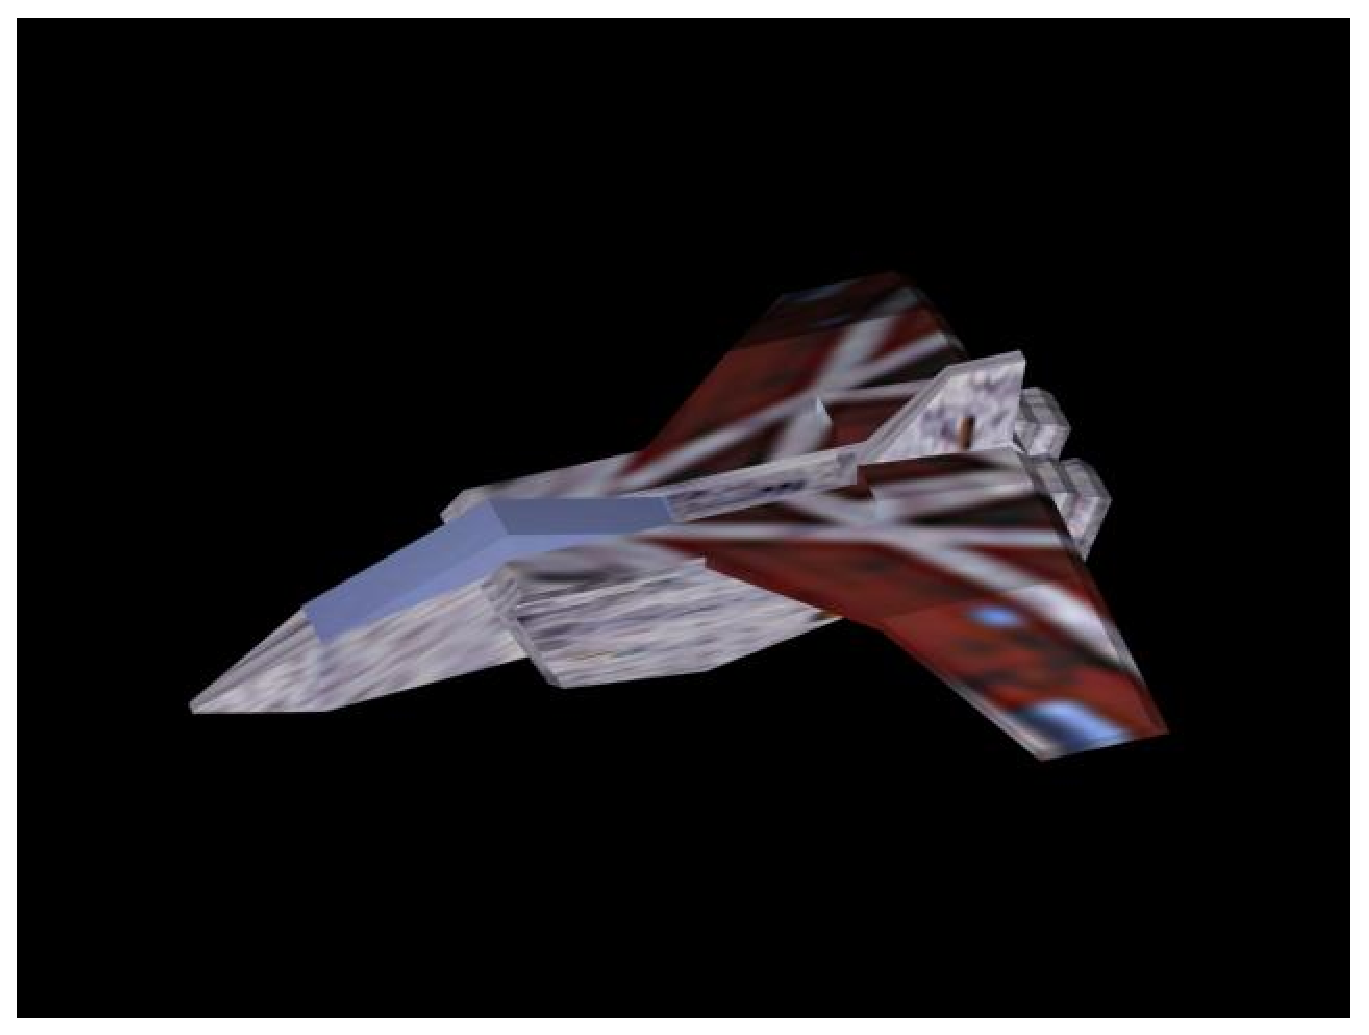
\includegraphics[width=10cm]{image001.eps}
\caption{Før Mesh Smooth}
\end{figure}

\begin{figure}[hbtp!]
\center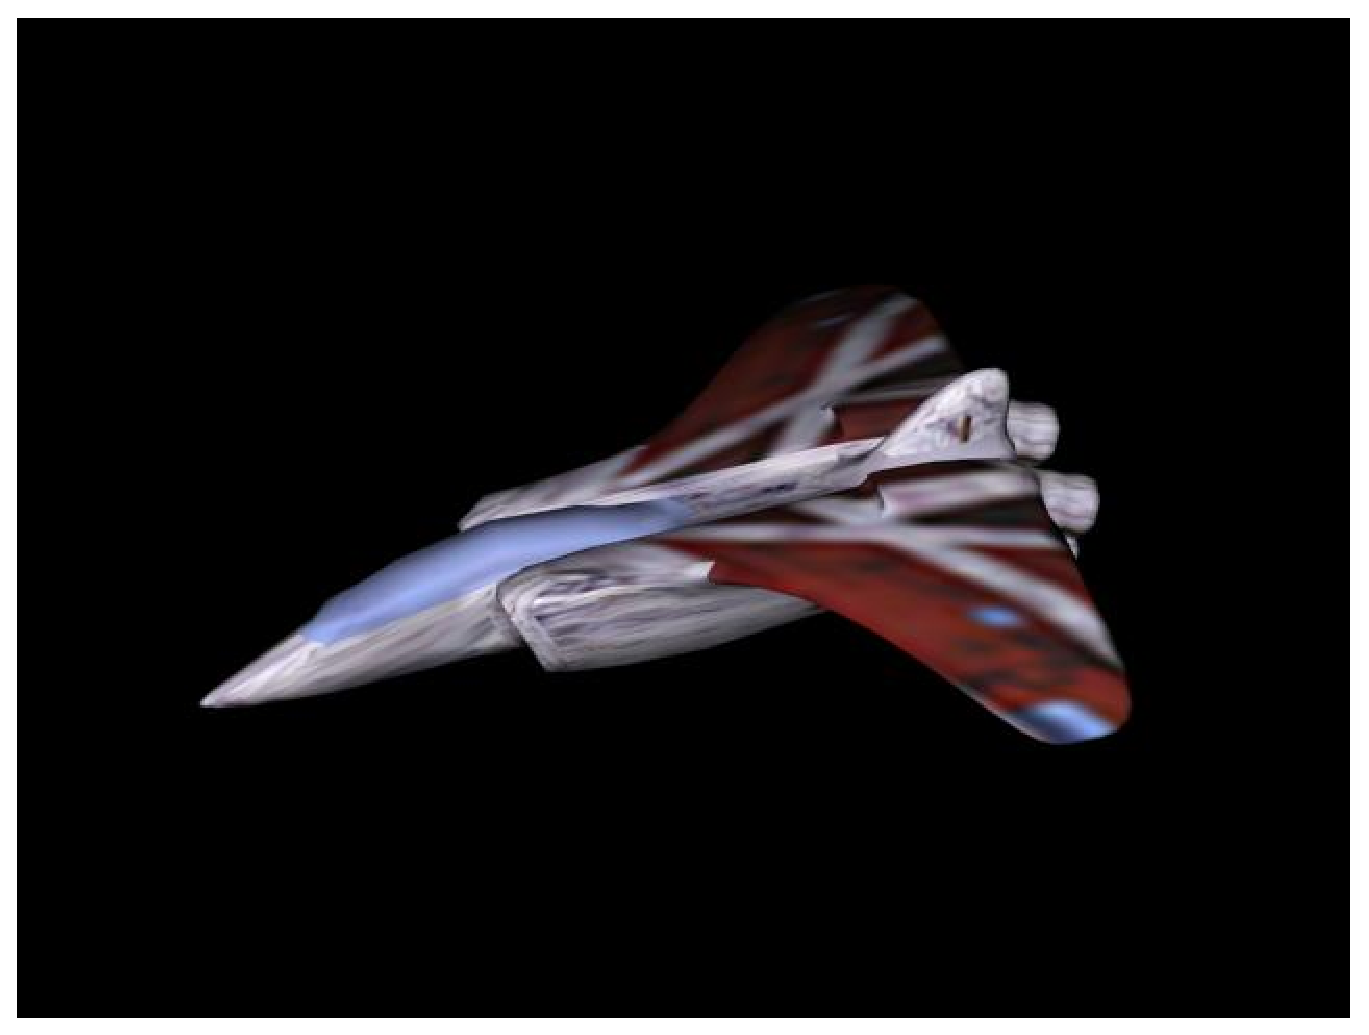
\includegraphics[width=10cm]{image003.eps}
\caption{Etter Mesh Smooth}
\end{figure}

En ganske viktig del som nå skulle lages var selve brettet som skipet
skulle fly gjennom. Vi kom til enighet om at det skulle se ut som en
hule vi fløy gjennom.

For å løse dette lagde jeg til sammen 29 tuber som jeg modifiserte.
For å lage overganger fra tynne tuber til tjukkere tuber brukte jeg
modifieren taper. For det meste ble bend brukt for å lage litt svinger
i hulen.

Det største problemet under lagingen av brettet var å få tettet igjen
overgangene mellom hver tube. Det gikk greit i begynnelsen, men
etterhvert som brettet ble større ble det vanskeligere og vanskeligere
å zoome inn skikkelig for å se. Løsningen vi kom fram til ble ganske
tungvinn og tidkrevende: Tubene ble eksportert en etter en og deretter
import inn i spillet slik at en kunne sjekke om det var sprekker der.
Det ble ganske mye ekpsortering og importering ettersom dette måtte
gjøres for hver forandring.

Da vi hadde fått et tilfredstillende resultat brukte jeg modifieren
noise for at ikke hele hulen skulle ha rette vegger. Resultat ble
veldig bra etter min mening, men da dukket problemet med sprekker i
overgangene opp igjen. Siden dette ikke var veldig synlig unntatt ved
visse vinkler lot vi det gå.

Teksturene som ble brukt på brettet ble funnet på internett og i
teksturlageret til 3ds max. Det ble såklart nok en gang problemer når
teksturene skulle legges på. Hvis teksturene bare ble lagt rett på ble
de strukket ut over hele objektet, og siden objektene var ganske store
så det ikke særlig bra ut.

Løsningen på dette ble å definere uvw koordinatene selv på hver tube.
Jeg skalerte opp alle punktene slik at teksturen ble lagt mange ganger
ved siden og over hverandre. Da dukket det opp nok et problem der det
på visse teksturer ble klare overganger der de ble lagt etter
hverandre. For å løse dette måtte jeg bare bruke teksturer der kantene
så noenlunde like ut slik at det skulle se ut som én stor tekstur når
flere ble lagt ved siden av hverandre evt. klippe ut deler av et
bilde.

\begin{figure}[!hbtp]
\center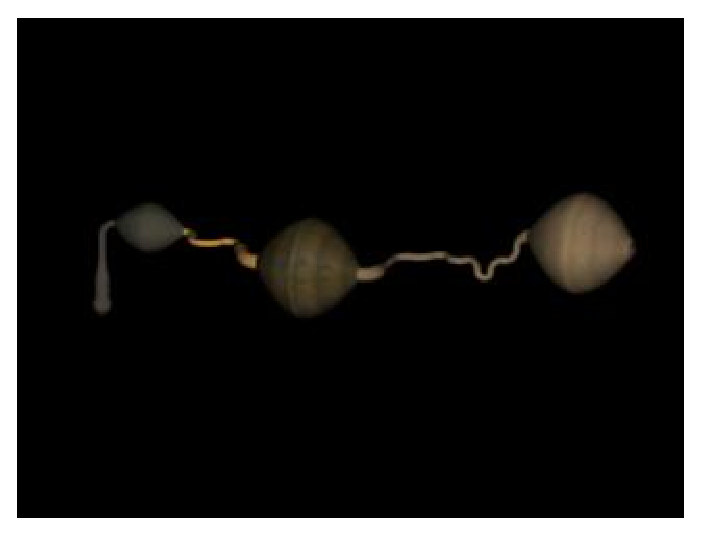
\includegraphics[width=10cm]{image005.eps}
\caption{Brettet fra utsiden}
\end{figure}

De siste tingene som nå manglet var steiner(meteoritter) og
krystaller. For å lage steinene brukte jeg kuler med forskjellige
former og noise på for å få en bulkete overlflate. Teksturene ble
lagt på med samme teknikk som på brettet.

Krystallen var også grei å lage. Jeg lekte meg med forskjellige
modifiere på en kule, og lattice ga det tøffeste resultatet. Teksturen
ble laget av kunstneren selv i paint der jeg bare fargela et område
med en blågrønn farge.

\chapter{Lasting av modellene}\label{3dload}

Spilllets modeller ble tegnet i 3d-studio max. Vi trengte derfor en
måte å få 3dStudio-modellene fra 3dstudio og inn til vårt program, for
så å kunne flytte og manipulere på de forskjellige objektene. Vi søkte
rundt på internett, men kunne ikke finne en loader som vi kunne bruke
direkte i vårt programmerings-miljø SDL (Simple DirectMedia Layer),
C++ og Linux. Det vi fant brukte vi til å lage vår egen loader.

Når man jobber i 3dstudio-max lagres filene som *.max ,vi gikk ikke
inn på dette formatet, men eksporterte filene som *.3ds. Man får da en
binær-fil med informasjon om objektet. Formatet inneholder mye
informasjon som vi ikke hadde bruk for. Denne informasjonen leser
loaderen bare inn i minnet for så å slette den fra minnet. Den
informasjon vi trengte i vårt program var informasjon om punktene til
objektet, informasjon om flatene til objektet(indexer for oppslag i
punkttabellen), informasjon om texturen til objektet, filnavnet til
bitmap-filen og informasjon om hvordan texturen(bildet) skulle
plasseres på objektet.

Loaderen ble bygget som en klasse CModel3ds. Tanken med dette var å
gjøre det enklest mulig å laste inn objekter.Klassen har bare to
public funksjoner i tillegg til konstruktøren; Load() og Render(). Slik
klassen ble bygget er det nå mulig å instansiere og loade
(Cmodel3ds::Load()) Cmodel3ds-objektet i programmets init-funksjon. I 
programmets opptegningsfunksjon kalle Render (Cmodel3ds::Render())
for hver gang objektet skal tegnes opp.

3ds-filen er bygd opp av chunks og subchunks. En chunk inneholder
informasjon om hva som kommer videre i fila (ID) og hvor mange bytes
av informasjon denne chunken inneholder. Det loaderen gjør er å lese en
chunk for så å teste på ID-en om det er informajon vi trenger, hvis vi
ikke trenger informasjonen leser vi inn neste osv., til vi finner noe
vi trenger. Dette gjøres frem til fila er slutt.

Gjennom å lage denne loaderen fikk vi oss et par overraskelser.
3d-studio lagrer objektene med z-koordinaten pekende oppover, mens
OpenGL bruker y-koordinaten til oppover. Dette medfører at etterat vi
har lest inn punktene, må vi bytte z og y-koordinat og å gi z-koordinaten
motsatt fortegn for at objektet skal se likt ut i 3d-studio og
programmet vårt.  SDL lagrer bitmap opp ned i forhold til opengl, for
å få bildet riktig må bildet snus. SDL lagrer bitmap som BGR(blue,
green, red) mens opengl har vanlig RGB så rekkefølgen her må også
snus.  I tillegg har vi slitt med minne-feil(segmentation fault). Vi
fant til slutt ut at årsaken var en uinitialisert variabel. Det som
skjedde var at når vi leste inn to bytes inn i en int (4 bytes) kunne
en ikke være trygg på at denne variblen var 0 i starten. Det måtte den
være siden vi bare leser inn 2 bytes i en int (4 bytes). Noen ganger
fikk vi riktig mens andre ganger ikke ,så dette skaffet oss hodebry. De
to mest signifikante bytene kunne i prinsippet være hva som helst
etter å ha lest inn to bytes i de minst signifikante bytene i int-en.

\chapter{Kollisjonsdeteksjon}\label{collision}

Som nevnt i innledningen måtte vi (som de fleste andre
spillprodusenter) jukse når vi skulle takle temaet
kollisjonsdeteksjon. Det første vi gjorde, var å dele brettet inn i 30
segmenter, og lage en funksjon for å finne midtpunktet i hvert av
disse segmentene, og avstanden til det punktet i segmentet som lå
lengst unna dette senteret. Da kan vi tenke oss en kule rundt
segmentet med senteret som, ja, senter... og avstanden som radius i
kula. Denne kula vil da dekke segmentet helt. 

Denne teknikken utførte vi også på skipet. Dette gjorde jobben
vesentlig mindre, siden vi kan si følgende: Hvis summen av radiusene
til skipet og et gitt segment er mindre enn avstanden mellom senteret
til skipet og senteret til segmentet, vil skipet garantert \emph{ikke}
kollidere med segmentet.

Det betyr likevel ikke at det faktisk er en kollisjon hvis det hvis
denne summen er større enn avstanden mellom skip og segment. Hvis den
er det, må vi sjekke nøyere. Og da er det fortsatt ca 2000 * ca 2000 =
ca 4 millioner flater å teste på, som er \emph{mye}.

Løsningen ble å lage to versjoner av brettet og skipet. En som så flott ut, og
vi ville vise på skjermen, og en som hadde \emph{meget få} flater.
Flyet fikk der 1 flate, og de fleste brettene 32 eller 64 flater.
Algoritmen var nå forbedret flere titalls tusen ganger på bekostning av
litt nøyaktighet (men langt i fra tilsvarende tidsbesparelsen...).

Så kom det vanskelige: plan-plan-skjærings-testing. Her måtte jeg ty
til boka mi ``Game Programming Gems''. Først finner jeg planlikningen
til flate 1. Så lager jeg tre linjer utfra de 3 punktene i flate 2.
Beskriver dette som en parametrisk likning med variabel t, og tester
ved hvilken t-verdi linja krysser planet til flate 1. Hvis $t=\infty$, 
så er linja parallell til planet, og hvis $t\in[0,1]$, så treffer
linja der hvor flate 2 befinner seg.

Deretter må jeg sjekke om linja skjærer der flate 1 befinner seg.
Dette gjøres ved å redusere flate 1 og 2 til 2D, ved å droppe den
komponenten som har størst absoluttverdi i normalvektoren i flate 1.
Ved å fjerne den samme komponenten i skjæringspunktet, kan vi
sjekke om dette punktet er på innsida eller utsida av alle tre sidene
i flata ved å teste på fortegn og sammenlikne med fortegnet til
senteret i flata. Er punktet på innsiden av alle tre sidene, har vi en
kollisjon.

\chapter{Effekter}\label{fx}

\section{Lyd}

Vi hadde ikke så veldig mye tid til musikk og lydeffekter, men Tor
Arvid lagde et lite bakgrunnsspor, og en liten fanfare på slutten.
Eksplosjonslyd og plinge-lyd til krystallene fant vi på nettet.

SDL har veldig greie funksjoner for å laste lyder av alle slags kjente
formater (wav, mp3, ogg, mod, ...). Det er også lett å initialisere
lydkortet og spille av filene.

\section{Partikkeleksplosjon}

Spillet vårt trengte en reaksjon når flyet kræsjet med steiner eller
omgivelsene. Vi ville her prøve å simulere en eksplosjon.

Vi brukte samme teknikken som for loaderen, vi byggde også dette
partikkel-systemet som en egen klasse for at det skulle være lett å
bruke den i programmet, instansiere objektet i init og kalle
partikkel-systemets Render-metode i opptegningsfunksjonen.

Partikkel-systemet er bygget opp av mange små teksturer(en tekstur for
hver av partiklene) med en tilfeldig farge disse blir så spredd rundt
i en vilkårlig retning i rommet.Disse blir blendet med resten av
3d-verdenen ved at man slår av dybde-test (glDisable(GL\_DEPTH\_TEST))
og slår på blending (glEnable(GL\_BLEND)). I starten av en
eksplosjonen gis partiklene en tilfeldig farge (mest rødt, noe grønt,
og litt blått) slik at partiklenes farge blir mellom gul og rød. Vi
tar med litt blått slik at i starten av eksplosjonen når alle
elementene er samlet blir  senteret av eksplosjonen hvit. Eksplosjonen
starter med at man viser flere og flere partikler inntil alle er vist,
da spres alle partiklene i en vilkårlig retning i rommet.

For å sørge for at partiklene hele tiden vises mot kameraet har vi
brukt teknikken billboarding. Partiklene er ikke 3d-objekter, bare
flater som hele tiden rettes mot kameraet.For å få dette til må vi få
tak i view-matrisa ved glGet(GL\_MODELVIEV\_MATRIX, \&matrix). Deretter
bruker vi denne til å sørge for at alle flatene peker mot kameraet.

\chapter{Konklusjon}

Vi har i henhold til oppgavebeskrivelsen kommet ganske greit i mål.
Det største minuset er at spillet kjører helt uakseptabelt seint i
windows (ikke prøv det engang...). I begynnelsen ble det
(selvfølgelig) planlagt å ha velstrukturerte kodefiler... Dette gikk i
vasken ganske tidlig, og det er et eneste stort virvar. Mottoet ``If
it was hard to write, it should be hard to read'' passer kanskje
her.

Vi har lært masse gøy om OpenGL, 3D Studio, grafikk og programmering
generelt. Siden fagene på skolen lar en slippe unna med så mangt i
programmeringsveien, var dette en god sjanse til å prøve seg på et
skikkelig prosjekt.

Vi vil takke de nettsidene som har hjulpet oss å komme i gang, og de
som har hjulpet oss enten i samtale, eller over irc.

\chapter{Referanser}

\section{Internett}

{\tt http://nehe.gamedev.net\\
http://www.gametutorials.com}

\section{Bøker}
OpenGL Game Programming, Hawkins/Astle, 2001, Prima Tech
Publishing\\[1em]
Gane Programming Gems, DeLoura, 2000, Charles River Media

\end{document}
